\section{Implementation}

\subsection{Smart contract}

\subsubsection{Interface overview}

% TODO this is a bit weak

The contract interface is split into two, \href{https://github.com/MrHarrisonBarker/CRPL/blob/main/CRPL.Contracts/contracts/IStructuredOwnership.sol}{IStructuredOwnership.sol} which handles multi-ownership transactions and events and \href{https://github.com/MrHarrisonBarker/CRPL/blob/main/CRPL.Contracts/contracts/ICopyright.sol}{ICopyright.sol} which handles all \keyword{copyright} transactions and events (similar to the \href{https://eips.ethereum.org/EIPS/eip-721}{EIP-721} interface).

\begin{figure}[H]
\caption{ICopyright events}
\begin{lstlisting}[language=Solidity]
/// @dev Emits when a new address is approved to a copyright
event Approved(uint256 indexed rightId, address indexed approved);

/// @dev Emits when a new manager has been approved
event ApprovedManager(address indexed owner, address indexed manager, bool hasApproval);
\end{lstlisting}
\end{figure}

\begin{figure}[H]
\caption{IStructuredOwnership events}
\centering
\begin{lstlisting}[language=Solidity]
/// @dev Emits when a new copyright is registered
event Registered(uint256 indexed rightId, OwnershipStake[] to);

/// @dev Emits when a copyright has been restructured and bound
event Restructured(uint256 indexed rightId, RestructureProposal proposal);

/// @dev Emits when a restructure is proposed
event ProposedRestructure(uint256 indexed rightId, RestructureProposal proposal);

/// @dev Emits when a restructure vote fails
event FailedProposal(uint256 indexed rightId);
\end{lstlisting}
\end{figure}

If we first look at all the events defined most are simply explained and straight forward, \textit{Approved} and \textit{ApproveManager} are taken from the \nft standard (ApproveManager == ApprovalForAll) then for IStructuredOwnership I've introduced four new events enabling modifiable multi address ownership with consensus.


\begin{figure}[H]
\caption{IStructuredOwnership functions}
\centering
\begin{lstlisting}[language=Solidity]
/// @notice The current ownership structure of a copyright
/// @param rightId The copyright id
function OwnershipOf(uint256 rightId) external view returns (OwnershipStake[] memory);

/// @notice Proposes a restructure of the ownership share of a copyright contract, this change must be bound by all share holders
/// @param rightId The copyright id
/// @param restructured The new ownership shares
/// @param notes Any notes written concerning restructure for public record
function ProposeRestructure(uint256 rightId, OwnershipStake[] memory restructured) external payable;

/// @notice The current restructure proposal for a copyright
/// @param rightId The copyright id
/// @return A restructure proposal
function Proposal(uint256 rightId) external view returns (RestructureProposal memory);
    
function CurrentVotes(uint256 rightId) external view returns (ProposalVote[] memory);

/// @notice Binds a shareholders vote to a restructure
/// @param rightId The copyright id
/// @param accepted If the shareholder accepts the restructure
function BindRestructure(uint256 rightId, bool accepted) external payable;
\end{lstlisting}
\end{figure}

Then the four new and one modified functions to enable this functionality, \textit{ProposeRestructure} to propose a change of ownership and \textit{BindRestructure} to vote and come to consensus between the shareholders. \textit{OwnershipOf} is modified from \textit{ownerOf} from \nft which returns an address but now has to return a complex ownership structure.

\subsubsection{Registration}

Registration of a \keyword{copyright} as discussed in the \textit{Smart contract design} section uses the basic principles of existing contract implementations most importantly the \nft contract, which registers new tokens by assigning a wallet address as the result of a token's id in a mapping (hash table) stored on the contract. This is simple and secure as the resulting hash of a token id will always point to the same entry in the mapping and therefore address.

\begin{figure}[H]
\caption{Essential copyright mappings from \href{https://github.com/MrHarrisonBarker/CRPL/blob/main/CRPL.Contracts/contracts/Copyrights/CopyrightBase.sol}{CopyrightBase.sol}}
\centering
\begin{lstlisting}[language=Solidity]
// rightId -> ownership structures
mapping (uint256 => OwnershipStructure) internal _shareholders;
    
// rightId -> metadata
mapping(uint256 => Meta) internal _metadata;
\end{lstlisting}
\end{figure}

I've taken this design and modified it for my needs by mapping to a complex ownership structure instead of one address (enabling multi-ownership), I've then added a new mapping to save metadata (work hash, expiry date, legal protections) for each \keyword{copyright}. These technically could be merged into one mapping along with the four others, mapping from id to a larger more complex struct encompassing all data needed. However I wanted to keep the size of my data structures small with their own defined purpose, this also reduces transaction costs because only the data relevant is being processed.

\begin{figure}[H]
\caption{Register function from \href{https://github.com/MrHarrisonBarker/CRPL/blob/main/CRPL.Contracts/contracts/Copyrights/CopyrightBase.sol}{CopyrightBase.sol}}
\centering
\begin{lstlisting}[language=Solidity]
function Register(OwnershipStake[] memory to, Meta memory meta) public validShareholders(to) {
	
	uint256 rightId = _copyCount.next();

	// registering copyright across all shareholders
	for (uint256 i = 0; i < to.length; i++) {

		require(to[i].share > 0, INVALID_SHARE);

		_recordRight(to[i].owner);
		_shareholders[rightId].stakes.push(to[i]);
	}
        
	_metadata[rightId] = meta;
	_shareholders[rightId].exists = true;
        
	_approvedAddress[_copyCount.getCurrent()] = msg.sender;

	emit Registered(rightId, to);
	emit Approved(rightId, msg.sender);
}	
\end{lstlisting}
\end{figure}

As you can see from the above registration is straightforward: generate the next id, iterate over all shareholders inputted, add each shareholder to the mapping checking each has some shares, add metadata to mapping, approve the sender for this \keyword{copyright} and emit a registered and approved event to let my system know whats happened.

Lastly I want to focus on line 8, \textit{require} is apart of \textbf{Solidity}'s error handling. The \keyword{EVM} runs all functions transactionally in the programming sense meaning all changes to the persistent data structure are processed and saved after the function has completed successfully. This is extremely useful and greatly simplifies error handling because if we encounter an error no underlying changes to the data have taken place and the transaction simply fails. 

\textit{Require} therefore simply checks an expression is true and if not an error is thrown with a stated reason the transaction is canceled and no changes to any stored data structure are made. These are used throughout my \keyword{smart contract} to validate input data, I talk more about these in the \textit{Modifiers} section below. This \textit{require} on line 8 is checking all shareholders have more than zero shares otherwise throw and error with the reason "INVALID\_SHARE".

The events emitted from this function are "listened" to and processed in the back-end more information in the \textit{Blockchain event listeners} section below.

\subsubsection{Ownership restructure}

As discussed in the design of my \keyword{smart contract} I had to build a shareholder consensus function for making changes to the \keyword{copyright}, therefore changing the ownership structure is split into two functions/steps, first you propose a new structure then each shareholder must vote or \textit{"bind"} the new structure, when all the shareholders have agreed to the new structure mappings are updated to reflect the new ownership.

\begin{figure}[H]
\caption{ProposeRestructure function from \href{https://github.com/MrHarrisonBarker/CRPL/blob/main/CRPL.Contracts/contracts/Copyrights/CopyrightBase.sol}{CopyrightBase.sol}}
\centering
\begin{lstlisting}[language=Solidity]
function ProposeRestructure(uint256 rightId, OwnershipStake[] memory restructured) external override validId(rightId) isExpired(rightId) validShareholders(restructured) isShareholderOrApproved(rightId, msg.sender) payable {
        
        for (uint256 i = 0; i < restructured.length; i++) {

            require(restructured[i].share > 0, INVALID_SHARE);

            _newHolders[rightId].stakes.push(restructured[i]);
            _newHolders[rightId].exists = true;
        }   

        emit ProposedRestructure(rightId, _getProposedRestructure(rightId));
    }	
\end{lstlisting}
\end{figure}

Above is the first step of restructuring the proposal, this is a small function that simply iterates through all the new shareholders and added their address and shares to a new mapping called \textit{\_newHolders} which is the same as the \textit{\_shareholders} mapping and is there to hold proposed ownership structures before they're "bound". An event is emitted which tells the back-end that the proposal has been saved to the chain and to start accepting votes from owners.

\begin{figure}[H]
\caption{BindRestructure function from \href{https://github.com/MrHarrisonBarker/CRPL/blob/main/CRPL.Contracts/contracts/Copyrights/CopyrightBase.sol}{CopyrightBase.sol}}
\centering
\begin{lstlisting}[language=Solidity]
function BindRestructure(uint256 rightId, bool accepted) external override validId(rightId) isExpired(rightId) isShareholderOrApproved(rightId, msg.sender) payable 
{
	_checkHasVoted(rightId, msg.sender);
     
	// record vote
	_proposalVotes[rightId].push(ProposalVote(msg.sender, accepted));
	_numOfPropVotes[rightId] ++;

	for (uint256 i = 0; i < _proposalVotes[rightId].length; i ++) 
	{
		if (!_proposalVotes[rightId][i].accepted) 
		{
			_resetProposal(rightId);
			emit FailedProposal(rightId);

			return;
		}
	}

	// if the proposal has enough votes, **** 100% SHAREHOLDER CONSENSUS ****
	if (_numOfPropVotes[rightId] == _numberOfShareholder(rightId)) {
            
		// proposal has been accepted and is now binding

		OwnershipStake[] memory oldOwnership = OwnershipOf(rightId);
            
		// reset has to happen before new shareholders are registered to remove data concerning old shareholders
		_resetProposal(rightId);

		_shareholders[rightId] = _newHolders[rightId];

		delete(_newHolders[rightId]);

		emit Restructured(rightId, RestructureProposal({oldStructure: oldOwnership, newStructure: OwnershipOf(rightId)}));
	}
}	
\end{lstlisting}
\end{figure}

Now looking at the more complex \textit{BindRestructure} function: first the address is checked if they've voted already, the vote is then recorded in a new mapping \textit{\_proposalVotes}, all votes are checked, if any of the votes are false then the whole proposal is rejected, checks if all the shareholders have voted, if all the votes are in set \textit{\_shareholders} to the proposed structure from \textit{\_newHolders} and emit an event.
\br
This is a point of possible future development or discussion, for a proposal to be \textit{"bound"} a unanimous vote is needed however this system could take advantage of the distribution of shares with only a majority of shares needed to make a change.

I decided to keep the voting unanimous over concerns of complexity (extension of development time was predicted) and a possible moral issues as to the possibilities of exploitation using this. An issue of exploitation is inherent to both implementations however a unanimous vote gives equal power of exploitation to every party whereas using shares would give more power to high staked parties.
 

\subsubsection{Modifiers}

Modifiers are pieces of code run at either end of a function call usually used to verify function parameters, I'm using them exclusively at the start of function calls to test addresses, ids and expiry. The design of a modifier usually consists of an assertion plus any processing needed on the data. 

\begin{figure}[H]
\caption{isShareholderOrApproved modifier from \href{https://github.com/MrHarrisonBarker/CRPL/blob/main/CRPL.Contracts/contracts/Copyrights/CopyrightBase.sol}{CopyrightBase.sol}}
\centering
\begin{lstlisting}[language=Solidity]
modifier isShareholderOrApproved(uint256 rightId, address addr) 
{
	uint256 c = 0;
	for (uint256 i = 0; i < _shareholders[rightId].stakes.length; i++) 
	{
		if (_shareholders[rightId].stakes[i].owner == addr) c ++;
	}
	require(c == 1 || _approvedAddress[rightId] == addr, NOT_SHAREHOLDER);
	_;
}
\end{lstlisting}
\end{figure}

This modifier is essential to authenticating a message sender is allowed to make changes to a specific \keyword{copyright} by checking it exists in ether \textit{\_shareholders} or \textit{\_approvedAddress} mappings.

\begin{figure}[H]
\caption{validAddress modifier from \href{https://github.com/MrHarrisonBarker/CRPL/blob/main/CRPL.Contracts/contracts/Copyrights/CopyrightBase.sol}{CopyrightBase.sol}}
\centering
\begin{lstlisting}[language=Solidity]
modifier validAddress(address addr)
{
	require(addr != address(0), INVALID_ADDR);
	_;
}
\end{lstlisting}
\end{figure}

\keyword{Ethereum} has a reserved address called the \textit{zero-address} which is only used for \keyword{smart contract} creation transactions, this means it's good practice to check all the addresses the contract handles are not the \textit{zero-address}. 

\begin{figure}[H]
\caption{isExpired modifier from \href{https://github.com/MrHarrisonBarker/CRPL/blob/main/CRPL.Contracts/contracts/Copyrights/CopyrightBase.sol}{CopyrightBase.sol}}
\centering
\begin{lstlisting}[language=Solidity]
modifier isExpired(uint256 rightId)
{
	require(_metadata[rightId].expires > block.timestamp, EXPIRED);
	_;
}
\end{lstlisting}
\end{figure}

\keyword{Copyright} expiry is handled with a modifier instead of an explicit state change as it's not feasible to have a timed process that runs when the expiry time is hit because of the time scale \keyword{copyright} works in. Therefore every time a transaction interacts with a \keyword{copyright} the expiry time is checked against the current block timestamp throwing an error code if expired.

\subsection{Back-end}

The back-end comprises of an \textbf{ASP.NET} API and static file server, the API is comprised of controllers that depend on services which hold business logic.

\begin{figure}[H]
\caption{HTTP request generic data flow}
\centering
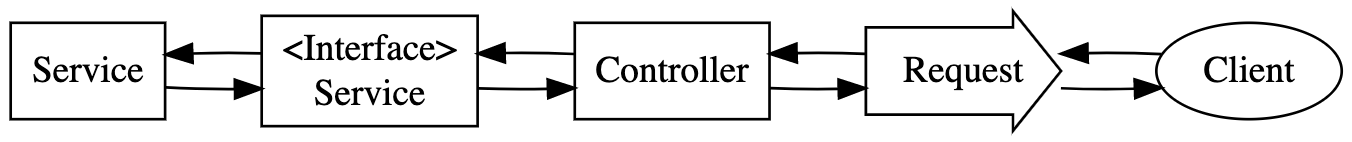
\includegraphics[width=\textwidth,height=\textheight,keepaspectratio]{images/patterns/service-controller}
\end{figure}

\subsubsection{API overview}
\begin{figure}[H]
\caption{Forms controller endpoints}
\centering
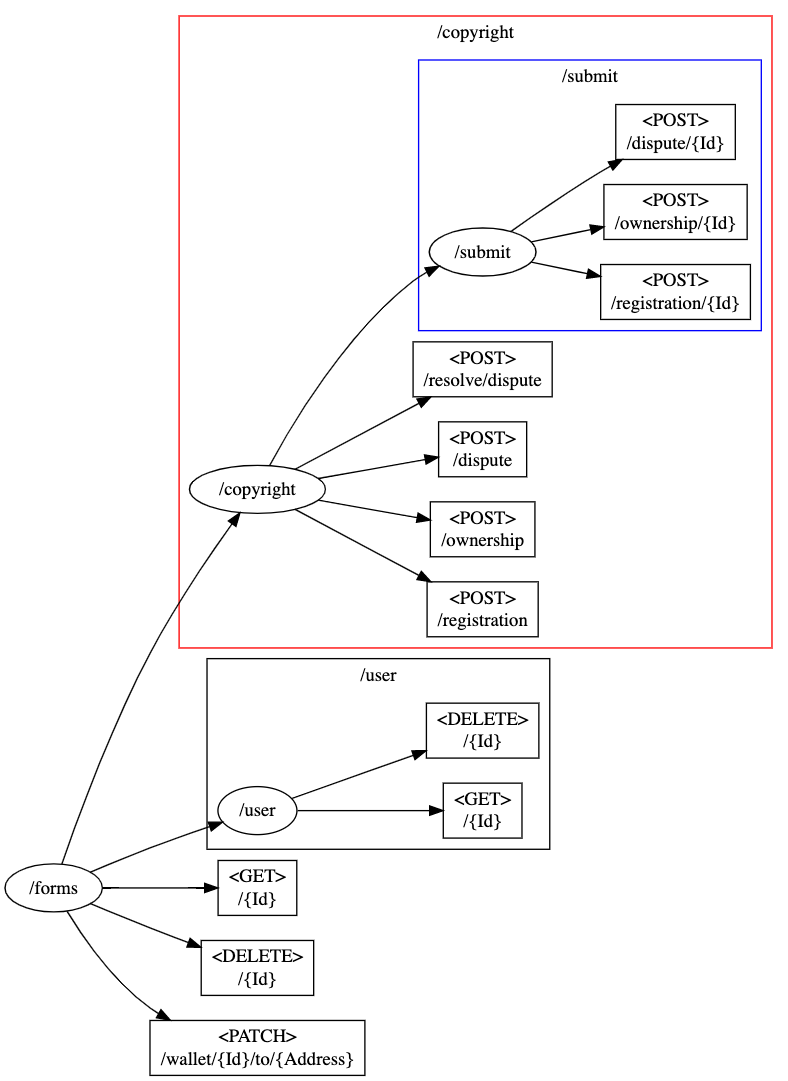
\includegraphics[width=\textwidth,height=0.5\textheight,keepaspectratio]{images/operational/Forms-Api}
\end{figure}

looking at the most complex and largest controller, I tried to keep the controller as \textit{RESTful} as possible with all endpoints describing the resource being accessed in conjunction with appropriate HTTP methods that describe the action performed on a resource.

\subsubsection{Applications framework}

The applications framework was built exploiting object oriented programming techniques mainly inheritance and polymorphism. An application has three classes each an implementation of each abstract base class, this means applications can be handled together generically and individually based on the child class.

\begin{figure}[H]
\caption{Application base class \href{https://github.com/MrHarrisonBarker/CRPL/blob/main/CRPL.Data/Applications/DataModels/Application.cs}{derived from}}
\centering
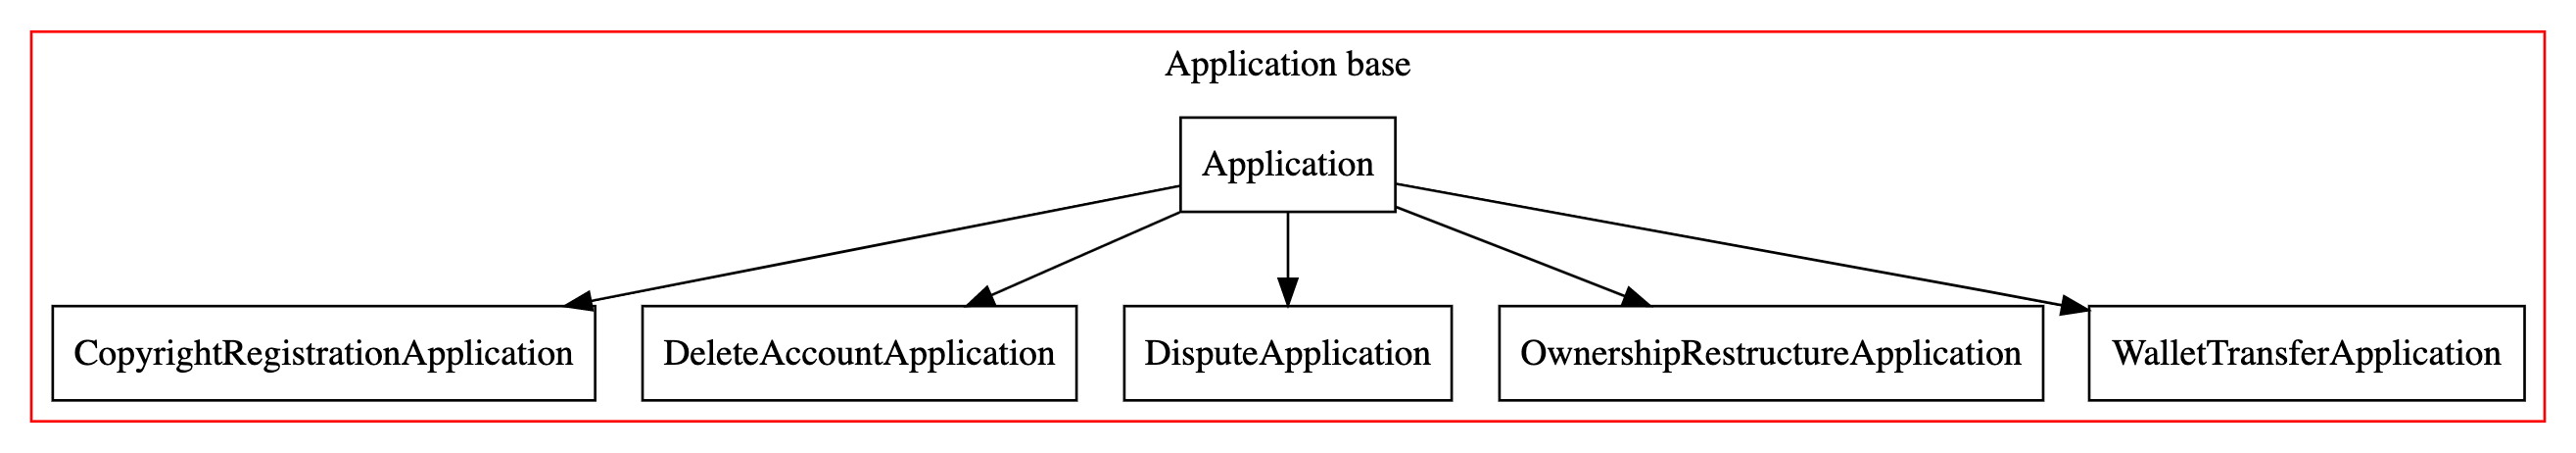
\includegraphics[width=\textwidth,height=0.5\textheight,keepaspectratio]{images/operational/application-base}
\end{figure}

This is the base \textit{Application} class and used by \textbf{EF Core} to generate database migrations creating and modifying tables. Therefore this class establishes all relationships, in this case a many to many with users and one to many with a registered work.

\begin{figure}[H]
\caption{Application view model class \href{https://github.com/MrHarrisonBarker/CRPL/blob/main/CRPL.Data/Applications/ViewModels/ApplicationViewModel.cs}{derived from}}
\centering
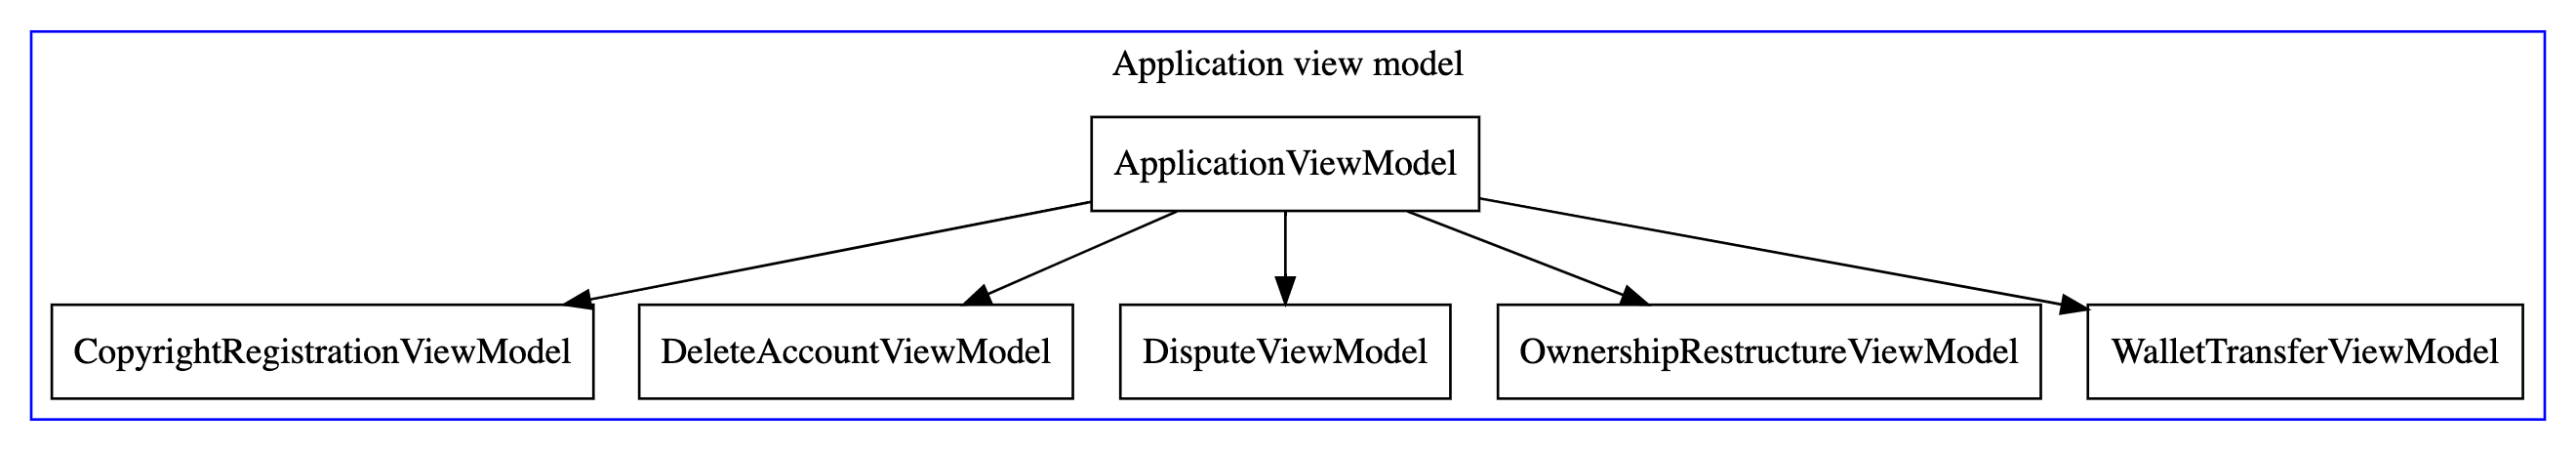
\includegraphics[width=\textwidth,height=0.5\textheight,keepaspectratio]{images/operational/application-view}
\end{figure}

The application view model is used when retrieving and displaying data, a lot of the time you don't want to send everything from the base model to the client or some processing/mapping maybe wanted. For applications the relationship between users is mapped from a junction table into a list of \textit{UserAccountMinimalViewModel}s
 
\begin{figure}[H]
\caption{Application input model class \href{https://github.com/MrHarrisonBarker/CRPL/blob/main/CRPL.Data/Applications/InputModels/ApplicationInputModel.cs}{derived from}}
\centering
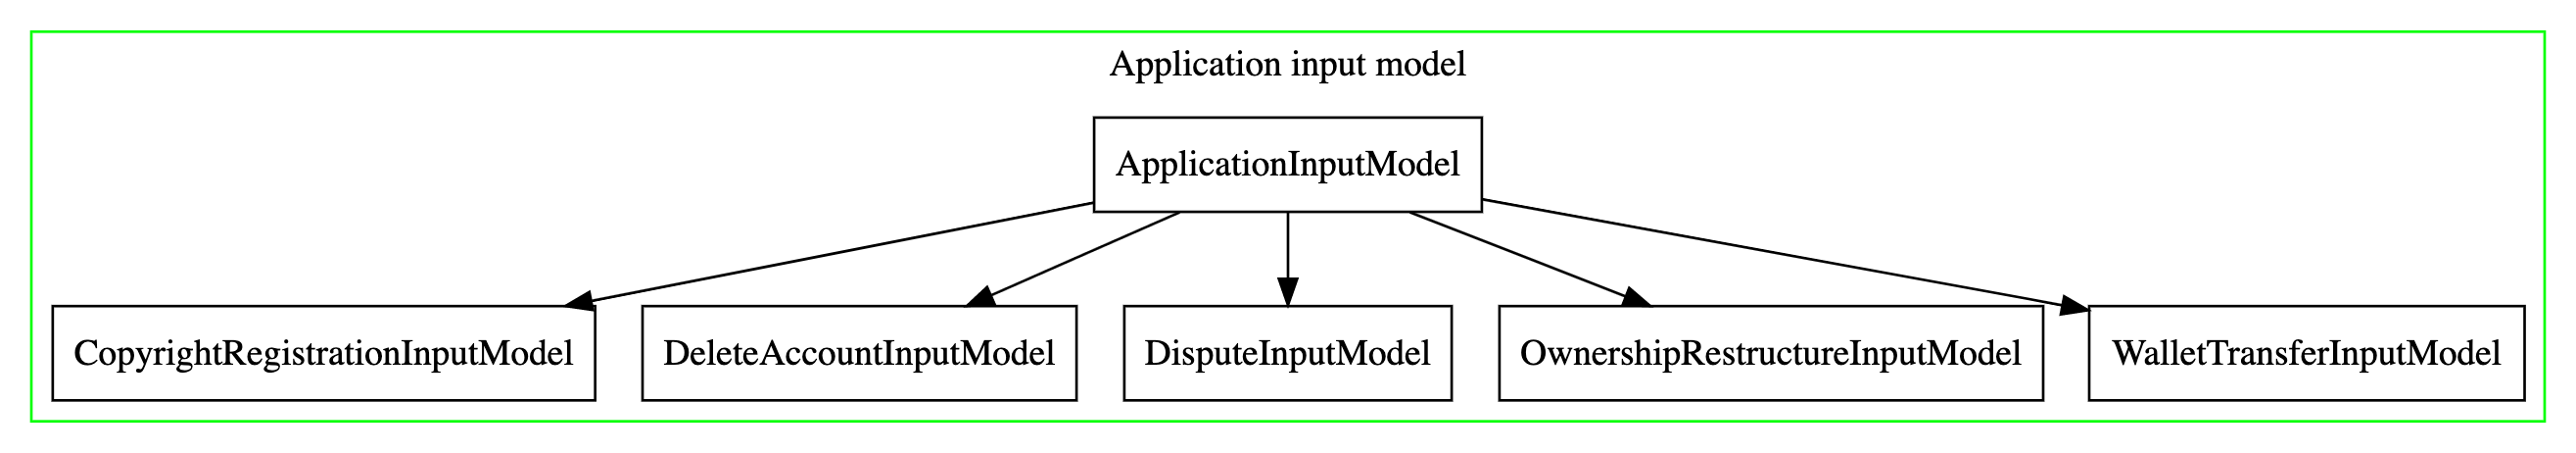
\includegraphics[width=\textwidth,height=0.5\textheight,keepaspectratio]{images/operational/application-input}
\end{figure}

Lastly an input model which is used when updating an application, this usually represents a real form the user is interacting with. This data is interpreted within the update method which modifies the data model on the database.
\br
One huge benefit of all applications using the same base class is that state can be generalised and kept consistent between different types of applications, a completed registration application should logically be the same as a completed dispute application.
This state can bee seen in the \textit{Applications framework} section of my design.

\begin{figure}[H]
\caption{Example application updater \href{https://github.com/MrHarrisonBarker/CRPL/blob/main/CRPL.Web/Core/Applications/Updaters/CopyrightRegistrationUpdater.cs}{CopyrightRegistrationUpdater}}
\centering
\begin{lstlisting}[language=CSharp]
public static class CopyrightRegistrationUpdater
{
    private static readonly List<string> Encodables = new() { "OwnershipStakes", "Id"  };
    
    public static async Task<CopyrightRegistrationApplication> Update(this CopyrightRegistrationApplication application, CopyrightRegistrationInputModel inputModel, IServiceProvider serviceProvider)
    {
        var userService = serviceProvider.GetRequiredService<IUserService>();
        
        application.UpdateProperties(inputModel, Encodables);

        if (inputModel.OwnershipStakes != null)
        {
            application.OwnershipStakes = inputModel.OwnershipStakes.Encode();

            application.CheckAndAssignStakes(userService, inputModel.OwnershipStakes);
        }

        return application;
    }
}
\end{lstlisting} 
\end{figure}

Each application also has an updater which is used for parsing the input model and updating the data model, this one is for the copyright registration application and is fairly simple. First it gets an instance of the user service, calls a static method I made that matches class properties between the input model and data model then updates those properties using the input model, complex object cant be saved in a db column so the ownership stakes are encoded into strings and then a relationship is updated/established between all the shareholders and the application.

\begin{figure}[H]
\caption{Example application submitter \href{https://github.com/MrHarrisonBarker/CRPL/blob/main/CRPL.Web/Core/Applications/Submitters/CopyrightRegistrationSubmitter.cs}{CopyrightRegistrationSubmitter}}
\centering
\begin{lstlisting}[language=CSharp]
public static class CopyrightRegistrationSubmitter
{
    public static async Task<CopyrightRegistrationApplication> Submit(this CopyrightRegistrationApplication copyrightRegistrationApplication, IServiceProvider serviceProvider)
    {
        var registrationService = serviceProvider.GetRequiredService<IRegistrationService>();
        
        await registrationService.StartRegistration(copyrightRegistrationApplication);

        copyrightRegistrationApplication.Status = ApplicationStatus.Submitted;
        
        return copyrightRegistrationApplication;
    }
}
\end{lstlisting}
\end{figure}

In addition to an updater applications need a submitter for when all the data has been inputted and is now ready to be processed, in the case of \textit{CopyrightRegistrationSubmitter} it starts the registration process (creates work and start verifying) and sets the status of the application to submitted. The majority of submitters start some background process or will require further processing to then be completed.

\subsubsection{Registration process}

The copyright registration process can be broken down into: fill and submit application, verification, send to chain and transaction verified.

\begin{figure}[H]
\caption{Registration state flow}
\centering
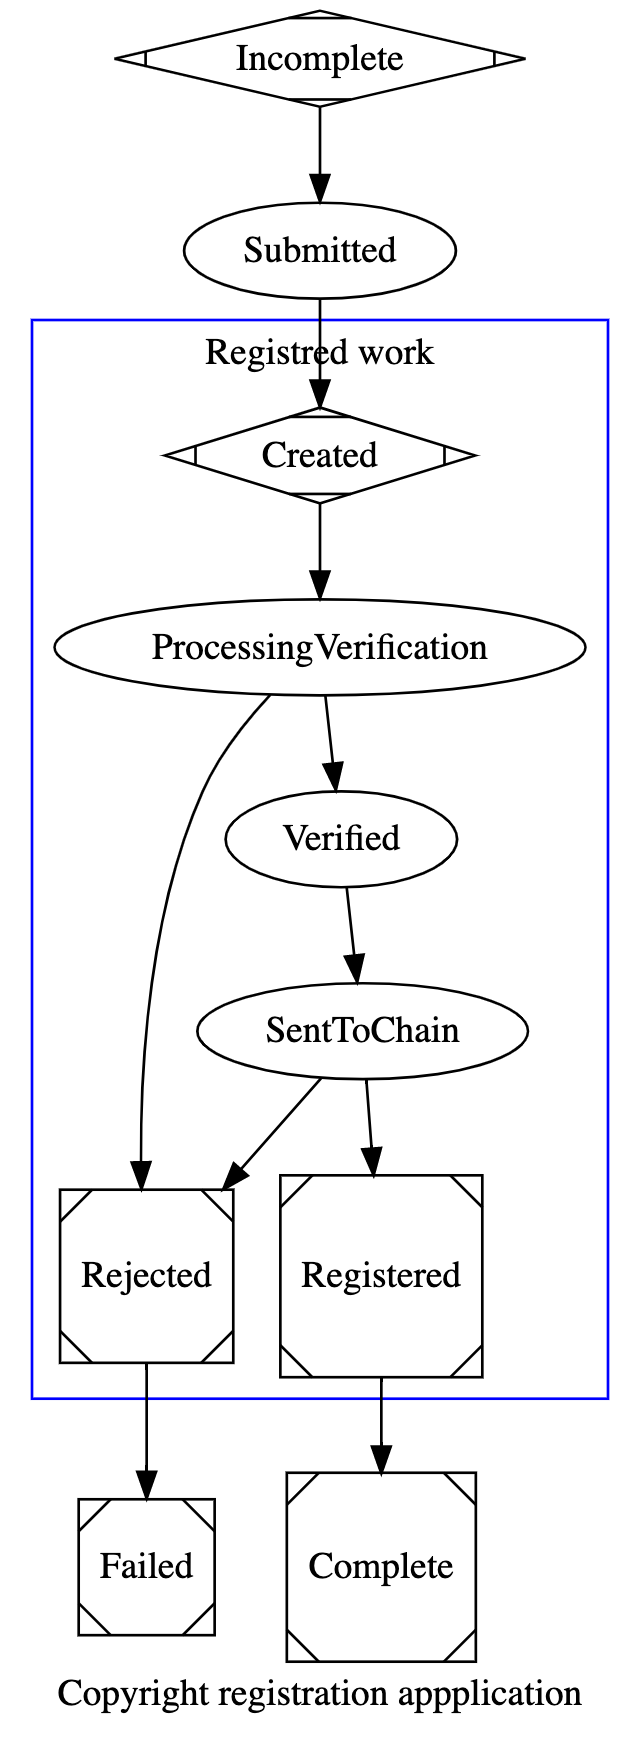
\includegraphics[width=\textwidth,height=0.5\textheight,keepaspectratio]{images/operational/cpy-registration-status-graph}
\end{figure}

The first step works as previously discussed, a user fills out a form/application submitting when all data has been inputted. validation of the data is handled on the client side with some server side sanity checks, this is reduce development workload and complexity however this is compromised by a user calling the API directly either maliciously or if I was to open up my API for public use.

% There is a section below talking about this step
\begin{figure}[H]
\caption{Finding collisions \href{https://github.com/MrHarrisonBarker/CRPL/blob/main/CRPL.Web/Services/WorksVerificationService.cs}{Line 57:58}}
\centering
\begin{lstlisting}[language=CSharp]
var collision = await Context.RegisteredWorks
           	.FirstOrDefaultAsync(x => x.Hash == work.Hash && x.Id != workId);
\end{lstlisting}
\end{figure}

Verification is handled by background service working though a queue which checks for collisions by comparing the uploaded work hash against all known work hashes. If a collision is found the application is set to \textit{Failed} and the work is set to \textit{Rejected}.

\begin{figure}[H]
\caption{Register message \href{https://github.com/MrHarrisonBarker/CRPL/blob/main/CRPL.Web/Services/RegistrationService.cs}{Line 88:102}}
\centering
\begin{lstlisting}[language=CSharp]
var register = new RegisterFunction()
{
	To = application.OwnershipStakes.Decode().Select(x => Mapper.Map<OwnershipStakeContract>(x)).ToList(),
	Meta = new Meta
	{
		Expires = new BigInteger((DateTime.Now.AddYears(application.YearsExpire) - new DateTime(1970, 1, 1, 0, 0, 0, DateTimeKind.Utc)).TotalSeconds),
		Title = application.Title,
		Registered = new BigInteger((DateTime.Now - new DateTime(1970, 1, 1, 0, 0, 0, DateTimeKind.Utc)).TotalSeconds),
		LegalMeta = application.Legal,
		WorkHash = Encoding.UTF8.GetString(application.WorkHash),
		WorkUri = application.WorkUri,
		WorkType = application.WorkType.ToString(),
		Protections = application.Protections
	}
};
\end{lstlisting}
\end{figure}

A \keyword{copyright} is then sent to the \keyword{blockchain} when a shareholder sends a complete request, this creates a register message (seen above) and sends it to the chain returning a transaction hash which is stored for later reference.

\begin{figure}[H]
\caption{Registered Event Processor \href{https://github.com/MrHarrisonBarker/CRPL/blob/main/CRPL.Web/Core/EventProcessors/RegisteredEventProcessor.cs}{Line 29:31}}
\centering
\begin{lstlisting}[language=CSharp]
context.Update(registeredWork);

registeredWork.RightId = registeredEvent.Event.RightId.ToString();
registeredWork.Registered = DateTime.Now;
registeredWork.Status = RegisteredWorkStatus.Registered;

registeredWork.AssociatedApplication.First(x => x.ApplicationType == ApplicationType.CopyrightRegistration).Status = ApplicationStatus.Complete;	
\end{lstlisting}
\end{figure}

Verifier and miner nodes on the network will now process this transactions, this takes an indeterminate time based on how much money you want to spend and the current capacity of the network. Once verified and processed into the chain a \textit{Registered} event will be picked up by the event processors running, the processor will match the transaction hashes setting the work to registered and its registration application to complete.

\subsubsection{Queries - Chain injection}

\begin{figure}[H]
\caption{Data injection from \keyword{blockchain} when querying registered works}
\centering
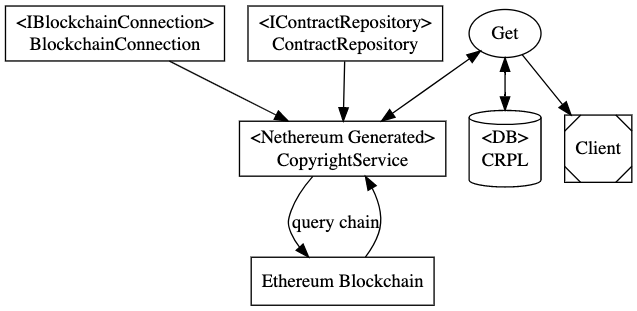
\includegraphics[width=\textwidth,height=\textheight,keepaspectratio]{images/operational/chain-inject}
\end{figure}

Because I rely on the \keyword{blockchain} as the store and point of truth in the system I need a way of querying a \keyword{copyright} for data to display to the user. 

\begin{figure}[H]
\caption{Metadata query from query service \href{https://github.com/MrHarrisonBarker/CRPL/blob/main/CRPL.Web/Services/QueryService.cs}{Line 155:156}}
\centering
\begin{lstlisting}[language=CSharp]
var meta = await new Contracts.Copyright.CopyrightService(BlockchainConnection.Web3(), ContractRepository.DeployedContract(CopyrightContract.Copyright).Address)
		.CopyrightMetaQueryAsync(rightId);
...
registeredWork.Meta = meta != null ? meta.ReturnValue1 : null;
\end{lstlisting}
\end{figure}

This is apart of a big function called \textit{injectFromChain} found in the \href{https://github.com/MrHarrisonBarker/CRPL/blob/main/CRPL.Web/Services/QueryService.cs}{query service} and is called whenever a work is requested from the service, it queries the \keyword{blockchain} for data then "injects" the found data into the existing registered work data model.

\subsubsection{Dispute handling}
% TODO filing disputes
% TODO resolving disputes: payment, change of ownership

\begin{figure}[H]
\caption{Dispute file and resolve flow diagram}
\centering
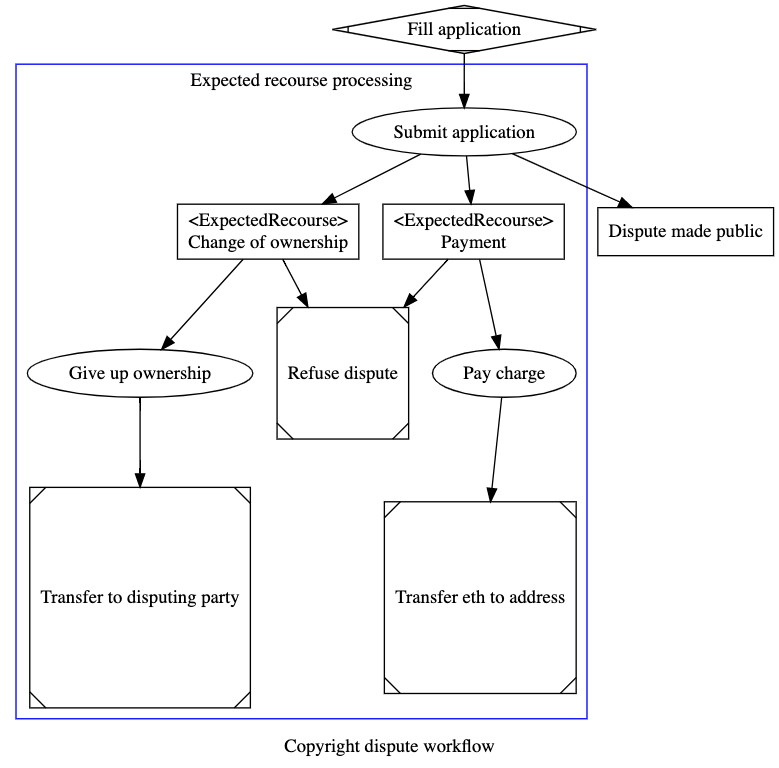
\includegraphics[width=\textwidth,height=\textheight,keepaspectratio]{images/operational/dispute-workflow}
\end{figure}

TODO

\subsubsection{Blockchain event listeners}

To listen for events in the \keyword{blockchain} \textbf{Nethereum} has a class called \textit{BlockchainProcessor} which listens for an event and registers a callback/action that is run when that specific event is found.

\begin{figure}[H]
\caption{Registering an event listener for \textit{Registered} event \href{https://github.com/MrHarrisonBarker/CRPL/blob/main/CRPL.Web/Services/Background/BlockchainEventListener.cs}{Line 32:33}}
\centering
\begin{lstlisting}[language=CSharp]
BlockchainConnection.Web3().Processing.Logs
	.CreateProcessorForContract<RegisteredEventDTO>(ContractRepository.DeployedContract(CopyrightContract.Copyright).Address, log => EventQueue.QueueEvent(log))
\end{lstlisting}
\end{figure}

For my system I'm using event processors that listen to a specific event type from a specific \keyword{smart contract}, see above this processor is listening for events of type \textit{RegisteredEventDTO} from the deployed contract retrieved from the \textit{ContractRepository}.

All my processors push all events to the event queue to be processed by a service instead of processing in the callback, this increases scaleability and breaks the code down into smaller modular chunks.

Events are pulled from the queue by the \href{https://github.com/MrHarrisonBarker/CRPL/blob/main/CRPL.Web/Services/Background/EventProcessingService.cs}{EventProcessingService} then processed by a \href{https://github.com/MrHarrisonBarker/CRPL/tree/main/CRPL.Web/Core/EventProcessors}{EventProcessor} which are static classes with one method \textit{ProcessEvent}, one is built for every event type listened to. 

\begin{figure}[H]
\caption{Processing events based on type \href{https://github.com/MrHarrisonBarker/CRPL/blob/main/CRPL.Web/Services/Background/EventProcessingService.cs}{Line 32:49}}
\centering
\begin{lstlisting}[language=CSharp]
switch (nextEvent.GetType().FullName)
{
	case var name when name.Contains("RegisteredEvent"):
		await ((EventLog<RegisteredEventDTO>)nextEvent).ProcessEvent(ServiceProvider, Logger);
		break;
	case var name when name.Contains("ApprovedEvent"):
		await ((EventLog<ApprovedEventDTO>)nextEvent).ProcessEvent(ServiceProvider, Logger);
		break;
	case var name when name.Contains("ProposedRestructureEvent"):
		await ((EventLog<ProposedRestructureEventDTO>)nextEvent).ProcessEvent(ServiceProvider, Logger);
		break;
	case var name when name.Contains("RestructuredEvent"):
		await ((EventLog<RestructuredEventDTO>)nextEvent).ProcessEvent(ServiceProvider, Logger);
		break;
	case var name when name.Contains("FailedProposalEvent"):
		await ((EventLog<FailedProposalEventDTO>)nextEvent).ProcessEvent(ServiceProvider, Logger);
		break;
}
\end{lstlisting}
\end{figure}

\subsubsection{Verification pipeline}

The verification pipeline uses by background service architecture with a \textit{VerificationQueue} and \textit{VerificationPipelineService} that dequeues and processes verification of a work. 

\begin{figure}[H]
\caption{Verification pipeline}
\centering
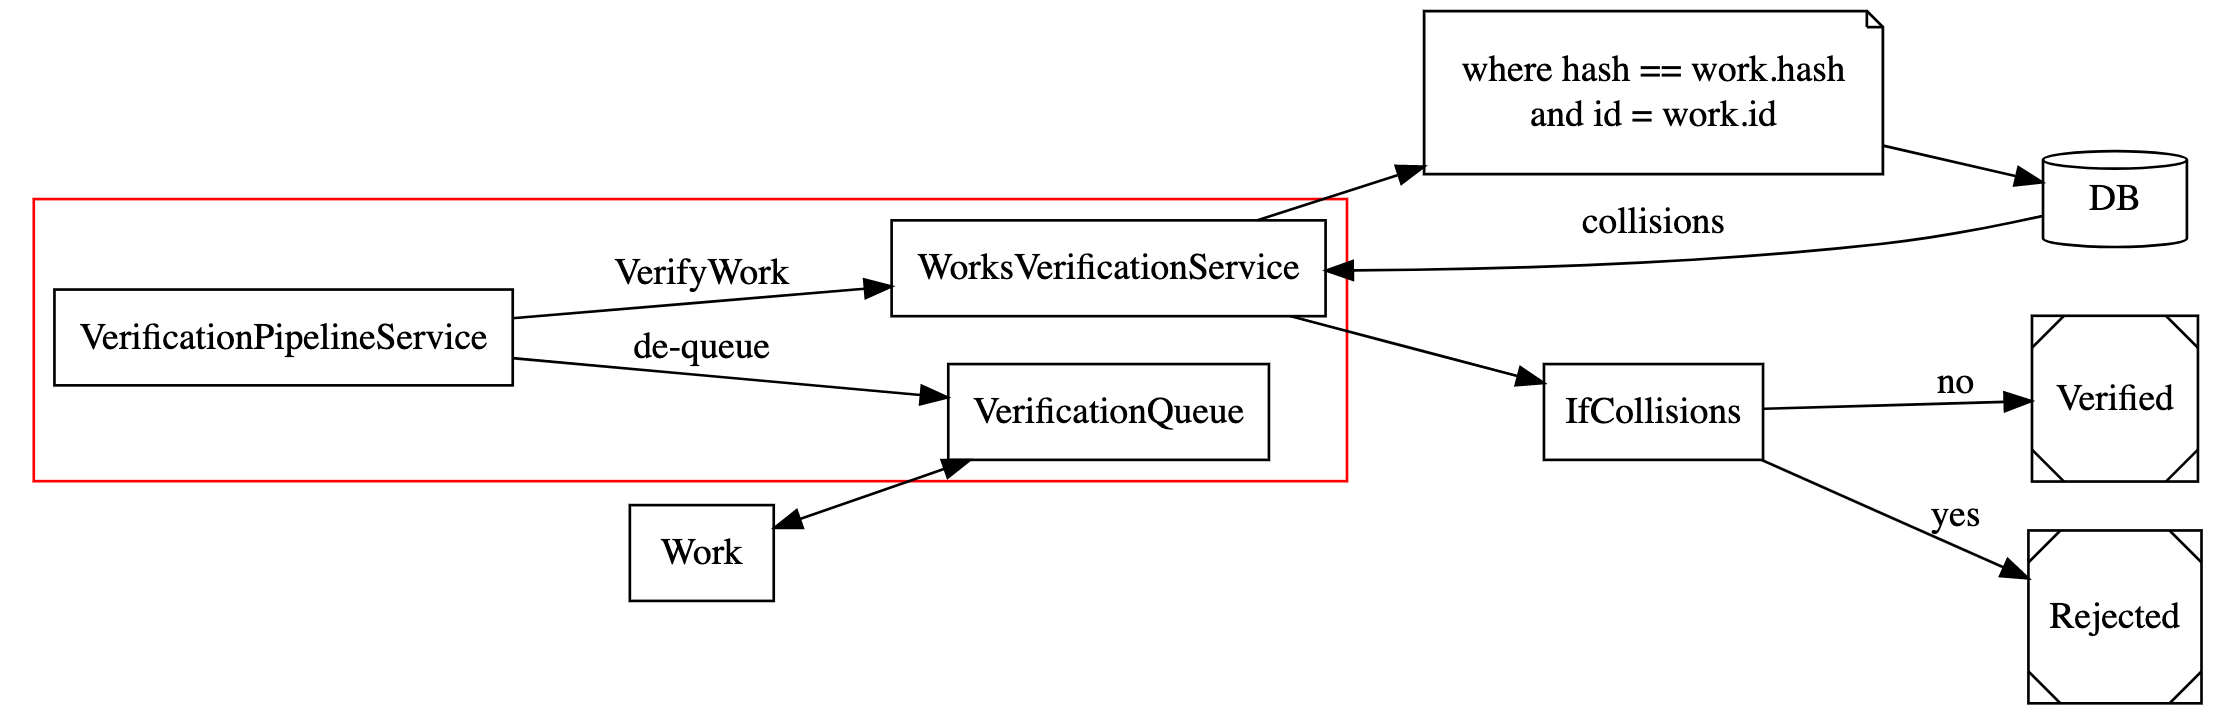
\includegraphics[width=\textwidth,height=\textheight,keepaspectratio]{images/operational/verification-pipe}
\end{figure}

% bit bad
When a work is pulled off the queue it is verified using the \href{https://github.com/MrHarrisonBarker/CRPL/blob/main/CRPL.Web/Services/WorksVerificationService.cs}{WorksVerificationService} method \textit{VerifyWork} which searches the database for existing works with the same hash. If no collisions are found the works status is updated to \textit{Verified}, if collision are found then the work is set to \textit{Rejected}

\begin{figure}[H]
\caption{hashing a work \href{https://github.com/MrHarrisonBarker/CRPL/blob/main/CRPL.Web/Services/WorksVerificationService.cs}{Line 146:151}}
\centering
\begin{lstlisting}[language=CSharp]
private byte[] HashWork(byte[] work)
{
	using var hashAlgorithm = SHA512.Create();

	return hashAlgorithm.ComputeHash(work);
}
\end{lstlisting}
\end{figure}

For hashing the uploaded work I stream the file into a byte array and compute the hash using \textbf{SHA-512} which has \(2^{512}\) total possible hash outputs which is \(1.34 \times 10^{154}\) almost double the number of atoms in the universe at around \(10^{82}\) so the possibility of a collision or exploitation is extremely low. 

Although \textbf{MD5} is mostly commonly used for very quick file duplicity checks these checks are usually just checksums to check file integrity of downloaded files. In terms of cryptographic security \textbf{SHA-512} is far better, \textbf{MD5} has been "broken" for years so should never be used for any sensitive or secure data hashing this is while the latest \textbf{SHA} algorithms are considered secure and are used in conjunction with "salt" for passwords in many systems.

\subsubsection{Account management}
% TODO issues with transfer and delete account
\subsubsection{Digital signing}
% TODO digital signing

\subsection{Database}

I've chosen to use a \textbf{MySQL} database for this project for two reasons: ease of use and \textbf{ACID}. Having previously used \textbf{MySQL} for multiple projects in the past plus the brilliant integration between \textbf{EFCore}, \textbf{LINQ} and \textbf{SQL}. \textbf{ACID} standing for \textbf{a}tomicity, \textbf{c}onsistency, \textbf{i}solation and \textbf{d}urability which ensure data integrity at the cost of speed over a \textit{NoSql} approach like \textbf{MongoDB}, it also has support for rigid relationships between entities.

\br

\label{sec:chainSync}
As talked about previously some data in the database has to be kept in parity with the \keyword{Blockchain} by querying the the deployed contract.

\begin{figure}[H]
\caption{ChainSync}
\centering
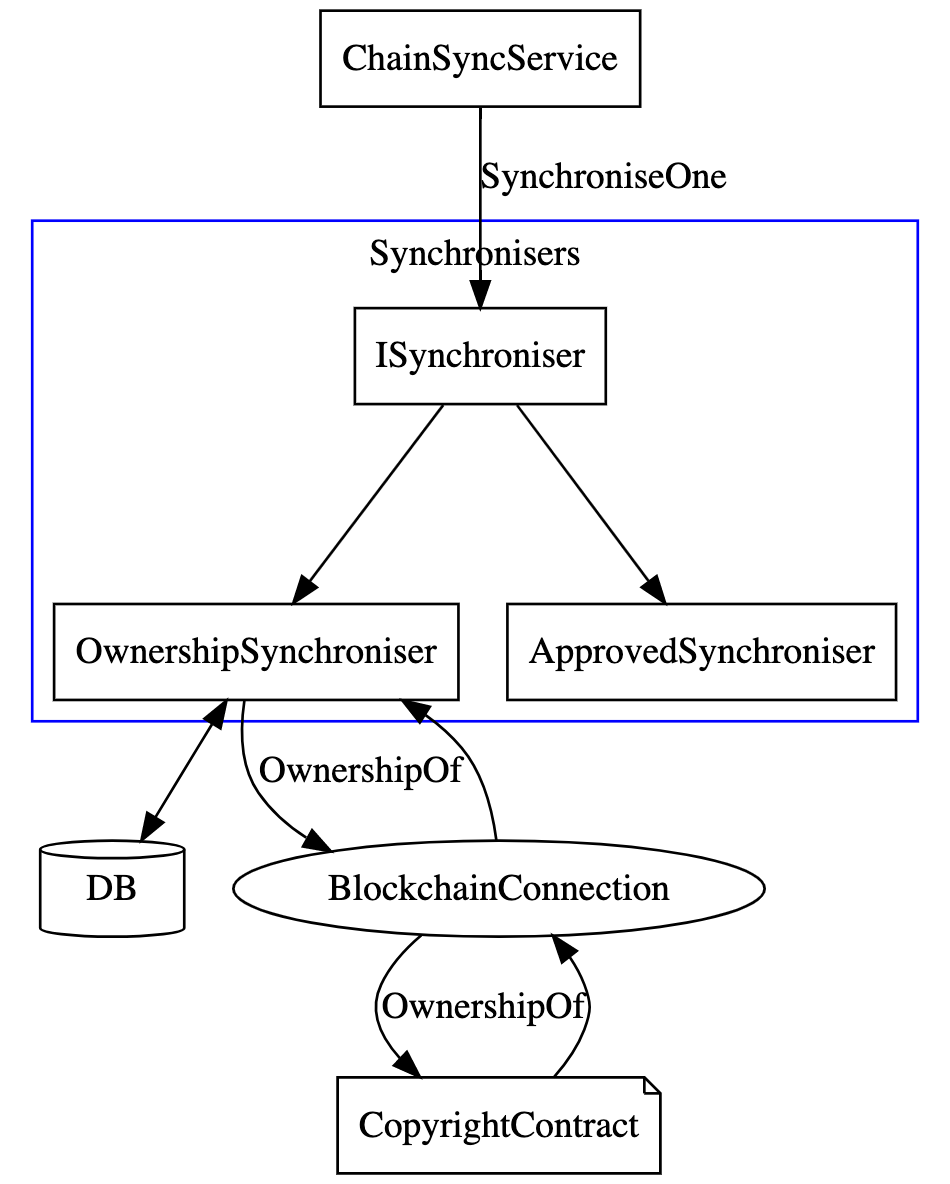
\includegraphics[width=\textwidth,height=0.5\textheight,keepaspectratio]{images/operational/chain-sync}
\end{figure}

Therefore a background service was built that synchronises all the \keyword{copyrights} currently being tracked with the \keyword{blockchain}, the service checks for changes on startup and then every 24 hours after startup.

\begin{figure}[H]
\caption{24 hour sync timer \href{https://github.com/MrHarrisonBarker/CRPL/blob/main/CRPL.Web/Core/ChainSync/ChainSyncService.cs}{Line 25:30}}
\centering
\begin{lstlisting}[language=CSharp]
CronTimer = new Timer(
	Sync,
	null,
	TimeSpan.Zero,
	TimeSpan.FromHours(24)
);
\end{lstlisting}
\end{figure}

There's only one synchroniser implemented in the system for ownership structures, it queries the \keyword{blockchain} using \textit{OwnershipOf} which is a method on the contract that returns an ownership structure for a specific \keyword{copyright}. It then checks against what is saved in the database, if changes are found relationships need to be removed and updated.

\begin{figure}[H]
\caption{ownership similarity \href{https://github.com/MrHarrisonBarker/CRPL/blob/main/CRPL.Web/Core/ChainSync/Synchronisers/OwnershipSynchroniser.cs}{Line 71, 77:86}}
\centering
\begin{lstlisting}[language=CSharp]
if (ownerships.Count != work.UserWorks.Count || !work.UserWorks.All(x => ownerships.Contains(x.UserAccount.Wallet.PublicAddress.ToLower())))
...
work.UserWorks.Clear();
ownerships.ForEach(async owner =>
{
	var user = await Context.UserAccounts.FirstOrDefaultAsync(x => x.Wallet.PublicAddress.ToLower() == owner.ToLower());
	if (user == null) throw new UserNotFoundException(owner);
	work.UserWorks.Add(new UserWork()
	{
		UserAccount = user
	});
});
\end{lstlisting}
\end{figure}

\subsection{Front-end}

A fancy UI was not a high priority of this project as the core back-end and \keyword{blockchain} interaction is expansive and complex enough in isolation, however I wanted to at least give a user the ability to interact with the system I've built hopefully in a usable and accessible way.

Most user interface design thought and work was spent on the four key forms (user register, copyright register, ownership restructure and dispute) as from previous experience forms are the hardest piece (for me) of interface design by far. To make this easier I counter intuitively at first did not care about the design or usability of the components I was building only getting the data into the form and sent off to the back-end.

This produced some initial designs that functionally work but were confusing for a new user and just didn't look very nice, I've found it's very easy to get hung up on user interface when building systems\footnote{I think this is down to the fact that it's the single point of contact with your users, most people will not see and or care about business logic code but how your interface looks and feels are front and centre. this would be okay in a real product development setting but for this project it's just not within the scope.} which slows down development especially in the early stages of development when the constraints and needs of the system are changing.

Then after all core features had been built I then went back to my forms and re-designed all input components using a consistent set of rules, requirements and style.    

\begin{figure}[H]
\caption{Example input markup \href{https://github.com/MrHarrisonBarker/CRPL/blob/main/CRPL.Web/ClientApp/src/app/Forms/cpy-registration-form/cpy-registration-form.component.html}{cpy-registration-form.component.html 9:18}}
\centering
\begin{lstlisting}[language=html]
<div class="input-container">
	<label class="input-label">Title<sup>*</sup></label>
	<div class="input-control">
	<input type="text" name="title" formControlName="Title" placeholder="Hello world"/>
	<div>This is a searchable title for the copyright, it doesn't have to be unique only descriptive and relevant&nbsp;<sup>*saved to the blockchain</sup></div>
		<clr-alert class="input-error" [clrAlertClosable]="false" clrAlertType="danger" *ngIf="InvalidAndUntouched('Title')">
		 	<clr-alert-item>This field is required!</clr-alert-item>
	 </clr-alert>
	</div>
</div>
\end{lstlisting}
\end{figure}

Below is the my \href{https://github.com/MrHarrisonBarker/CRPL/tree/main/CRPL.Web/ClientApp/src/app/Forms/ownership-structure-form}{ownership-structure-form} component that's used in both \href{https://github.com/MrHarrisonBarker/CRPL/tree/main/CRPL.Web/ClientApp/src/app/Forms/cpy-registration-form}{cpy-registration-form} and \href{https://github.com/MrHarrisonBarker/CRPL/tree/main/CRPL.Web/ClientApp/src/app/Forms/cpy-restructure-form}{cpy-restructure-form}, this means all forms have to be consistent across the application so any section of a form will "fit" into any other form.

\begin{figure}[H]
\caption{\href{https://github.com/MrHarrisonBarker/CRPL/tree/main/CRPL.Web/ClientApp/src/app/Forms/ownership-structure-form}{Ownership structure form} component}
\centering
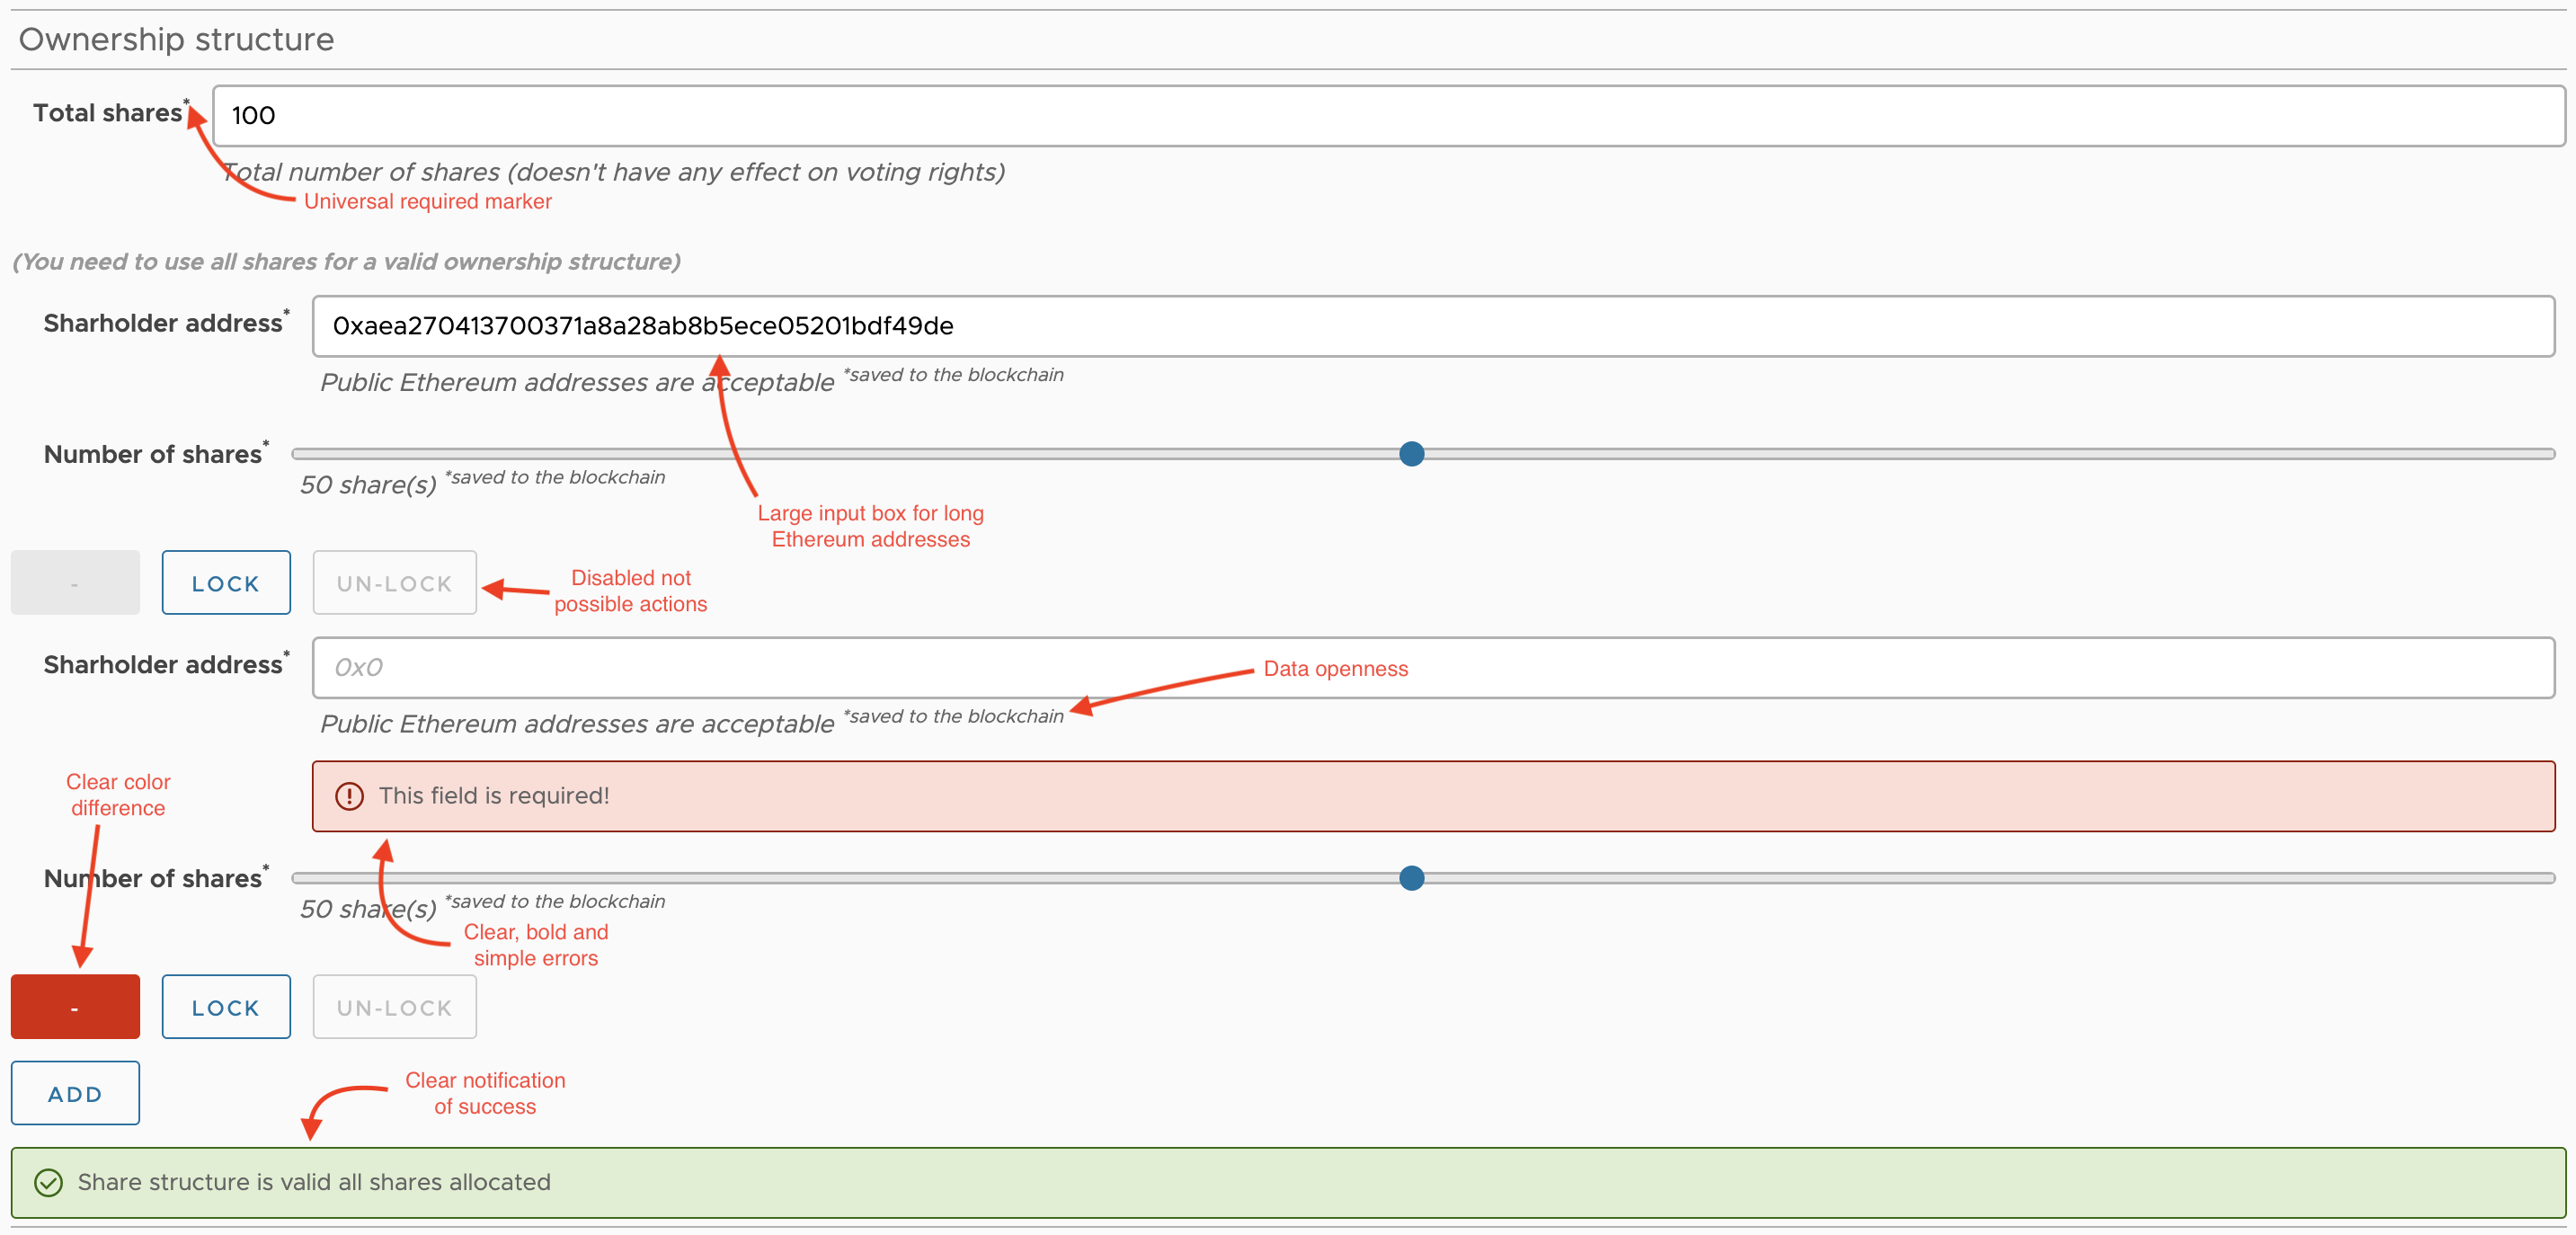
\includegraphics[width=\textwidth,height=\textheight,keepaspectratio]{images/wireframe/ownership-structure}
\end{figure}